% +------------------------------------------------------------------------+
% | Reference manual page: Linear_cell_complex_constructors.tex
% +------------------------------------------------------------------------+
% | 04.02.2010   Guillaume Damiand
% | Package: Linear_cell_complex
% +------------------------------------------------------------------------+
\ccRefPageBegin
%%RefPage: end of header, begin of main body
% +------------------------------------------------------------------------+

%----------------------------------------------------------------------------
\begin{ccRefFunction}{import_from_plane_graph<LCC>}
\ccInclude{CGAL/Linear_cell_complex_constructors.h}\\

\ccFunction{template<class LCC>
  typename LCC::Dart_handle import_from_plane_graph(LCC& lcc,
  std::istream& ais);}
{Imports an embedded plane graph read from \ccc{ais} into \ccc{lcc}. 
  Objects are added in \ccc{lcc}, existing darts are not modified.
  Returns a dart created during the import.
  \ccPrecond{\ccc{LCC::dimension}\mygeq{}2 and \ccc{LCC::ambient_dimension}==2.}
}

\ccHeading{File format} The file format must be the following.  First
the number of vertices and the number of edges of the planar graph.
Then, for each vertex of the planar graph, the coordinates of the
\myith{} vertex (two numbers for $x$ and $y$ coordinates). The first
vertex index is 0. Then for each edge of the planar graph, the two
indices of the two vertices (two numbers between 0 and the number of
vertices minus 1).

Here a small example:
\begin{verbatim}
5 6
1.0 3.0   0.0 2.0   2.0 2.0   0.0 0.0   2.0 0.0
0 1   0 2   1 2   1 3   2 4   3 4
\end{verbatim}
%
\def\LargFig{.5\textwidth}
  \begin{ccTexOnly}
    \begin{center}
      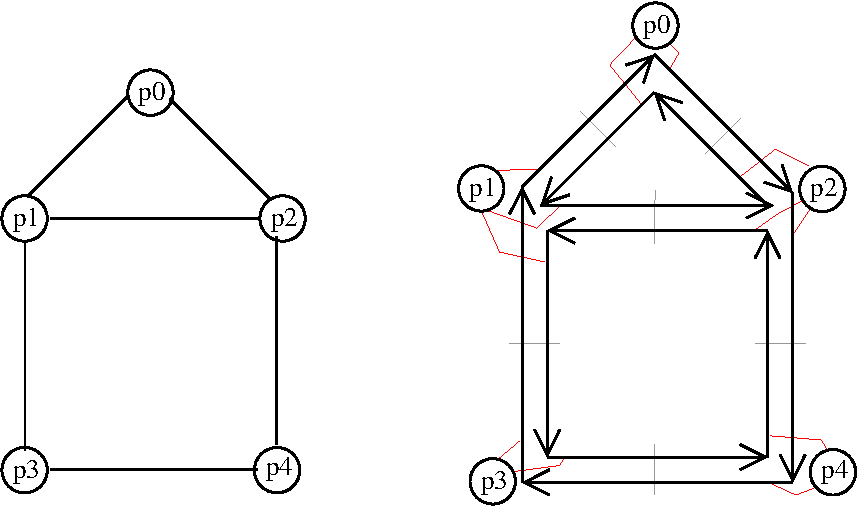
\includegraphics[width=\LargFig]{Linear_cell_complex_ref/fig/pdf/import_graph}
    \end{center}
  \end{ccTexOnly}
  \begin{ccHtmlOnly}
    <CENTER>
    <A HREF="fig/png/import_graph.png">
        <img src="../Linear_cell_complex_ref/fig/png/import_graph.png" alt=""></A>
    </CENTER>
    \end{ccHtmlOnly}
    \begin{center}
      Example of \ccc{import_graph} reading the above file as istream. \\
      \textbf{Left}: A planar graph embedded in the plane with 
      \emph{P0}=(1.0,3.0), \emph{P1}=(0.0,2.0), \emph{P2}=(2.0,2.0), \emph{P3}=(0.0,0.0), \emph{P4}=(2.0,0.0).
      \textbf{Right}: the 2D linear cell complex reconstructed.
      \end{center}
\ccSeeAlso
\ccRefIdfierPage{CGAL::import_from_triangulation_3<LCC,Triangulation>}\\
\ccRefIdfierPage{CGAL::import_from_polyhedron_3<LCC,Polyhedron>}

\end{ccRefFunction}
%----------------------------------------------------------------------------
\begin{ccRefFunction}{import_from_triangulation_3<LCC,Triangulation>}
\ccInclude{CGAL/Linear_cell_complex_constructors.h}\\

\ccFunction{template <class LCC,class Triangulation_>
   typename LCC::Dart_handle import_from_triangulation_3(LCC& lcc,
   const Triangulation_ &atr);}
 {Imports \ccc{atr} (a \ccc{Triangulation_3}) into \ccc{lcc}. 
   Objects are added in \ccc{lcc}, existing darts are not modified.
   Returns a dart created during the import.
  \ccPrecond{\ccc{LCC::dimension}\mygeq{}3 and \ccc{LCC::ambient_dimension}==3.}
 }
\ccSeeAlso
\ccRefIdfierPage{CGAL::import_from_plane_graph<LCC>}\\
\ccRefIdfierPage{CGAL::import_from_polyhedron_3<LCC,Polyhedron>}

\end{ccRefFunction}
%----------------------------------------------------------------------------
\begin{ccRefFunction}{import_from_polyhedron_3<LCC,Polyhedron>}
\ccInclude{CGAL/Linear_cell_complex_constructors.h}\\

\ccFunction{template<class LCC,class Polyhedron>
  typename LCC::Dart_handle import_from_polyhedron_3(LCC& lcc, 
                                       Polyhedron &apoly);}
{Imports \ccc{apoly} (a \ccc{Polyhedron_3}) into \ccc{lcc}. Objects are added in \ccc{lcc},
  existing darts are not modified.
  Returns a dart created during the import. 
  \ccPrecond{\ccc{LCC::dimension}\mygeq{}2 and \ccc{LCC::ambient_dimension}==3.}
}
\ccSeeAlso
\ccRefIdfierPage{CGAL::import_from_plane_graph<LCC>}\\
\ccRefIdfierPage{CGAL::import_from_triangulation_3<LCC,Triangulation>}

\end{ccRefFunction}
% +------------------------------------------------------------------------+
%%RefPage: end of main body, begin of footer
\ccRefPageEnd
% EOF
% +------------------------------------------------------------------------+
